\documentclass{article}

\usepackage{geometry}
\geometry{a4paper}
\setlength{\parindent}{10mm}
\setlength{\parskip}{0.9em}
\def\baselinestretch{1.5}

\usepackage[spanish,mexico]{babel}
\renewcommand {\spanishtablename}{Cuadro}
\usepackage[spanish,onelanguage,ruled]{algorithm2e}
\usepackage[utf8]{inputenc}
\usepackage{graphicx}
\usepackage{caption} 
\usepackage{amsmath}
\usepackage{amsthm, amsfonts}
\usepackage{enumerate} 
\usepackage{fancyhdr}
\usepackage{anysize} 
\usepackage[usenames]{color}
\usepackage{booktabs}
\usepackage{etoolbox}
\usepackage{fancyvrb}
\usepackage{color,soul}
\usepackage[dvipsnames]{xcolor}
\usepackage{graphicx}
 \usepackage{caption}
\usepackage{subcaption}
\usepackage{listings}
\usepackage{amssymb}
\usepackage{multirow}



\usepackage{verbatim}
% redefine \VerbatimInput
\RecustomVerbatimCommand{\VerbatimInput}{VerbatimInput}%
 {fontsize=\footnotesize,
  %
  frame=lines,  % top and bottom rule only
  framesep=1em, % separation between frame and text
  rulecolor=\color{Gray},
  %
  label=\fbox{\color{Black}test.txt},
  labelposition=topline,
  %
  %commandchars=\ \mid \(\), % escape character and argument delimiters for
                  % commands within the verbatim
  %commentchar=*        % comment character
 }


\pagestyle{fancy}

\chead{}
\lhead{} 
\rhead{}
\lfoot{\it }
\cfoot{}
\rfoot{\thepage}

\title{
\centering
Modelos Probabilistas Aplicados \\
Johanna Bolaños Zúñiga \\
Matricula: 1883900\\
Tarea 11
}

\date{}

\begin{document}
\maketitle

\section{Aplicación de la convolución}

La convolución es un operador matemático que transforma dos funciones en una tercera función que representa la magnitud en la que se superponen una función sobre una versión trasladada e invertida de la otra función. De acuerdo a Kim \cite{kim}, la convolución se puede describir como una función que es la integral (cuando las variables son continuas) o la suma de funciones (cuando las variables son discretas) de dos variables aleatorias independientes, y mide la cantidad de superposición cuando una función se desplaza sobre la otra. En las definiciones matemáticas la convolución, tanto discreta como continua, está indicada por el operador \textbf{$*$}.

En el procesamiento de señales digitales (DSP por sus siglas en inglés de \textit{digital signal processing}), donde una de sus aplicaciones prácticas son el tratamiento de las imágenes, en la que la convolución juega un papel importante, ya que es una técnica de procesamiento de imágenes común que cambia las intensidades de un píxel para reflejar las intensidades de los píxeles circundantes. Además, se puede obtener efectos de imagen populares como desenfoque, nitidez y detección de bordes \cite{developer}. Un detector de bordes puede procesar y extraer características relevantes en un conjunto de imágenes antes de que se introduzcan en un algoritmo de reconocimiento de patrones, lo que puede dar como resultado un rendimiento superior, por ejemplo, que un automóvil sin conductor frena en una señal de alto. La mejora de imágenes puede resultar especialmente útil cuando se trata de imágenes científicas. 

En el procesamiento de imágenes, muchas operaciones de filtro se aplican a una imagen realizando una operación especial llamada convolución con una matriz que recibe el nombre de kernel, los cuales son típicamente matrices cuadradas que van desde $2\times2$, hasta de $5\times5$, siendo la comúnmente utilizada la de $3\times3$. Los valores almacenados en el kernel se relacionan directamente con los resultados de la aplicación del filtro a la imagen y son los que determinan cómo transformar los píxeles de la imagen original en los píxeles de la imagen procesada \cite{developer}.

Dado que las imágenes también se pueden considerar como cuadrículas bidimensionales de números, la aplicación de un kernel a una imagen se puede visualizar como una pequeña cuadrícula (el kernel) que se mueve a través de una cuadrícula sustancialmente más grande (la imagen), donde la convolución del kernel hace que el valor de cada píxel se recalcula utilizando la suma de vecindad ponderada definida en la matriz del kernel. La representación de los pasos de esta convolución se puede observar en la figura \ref{convolucion1}.  

\begin{figure}[h]
    \centering
    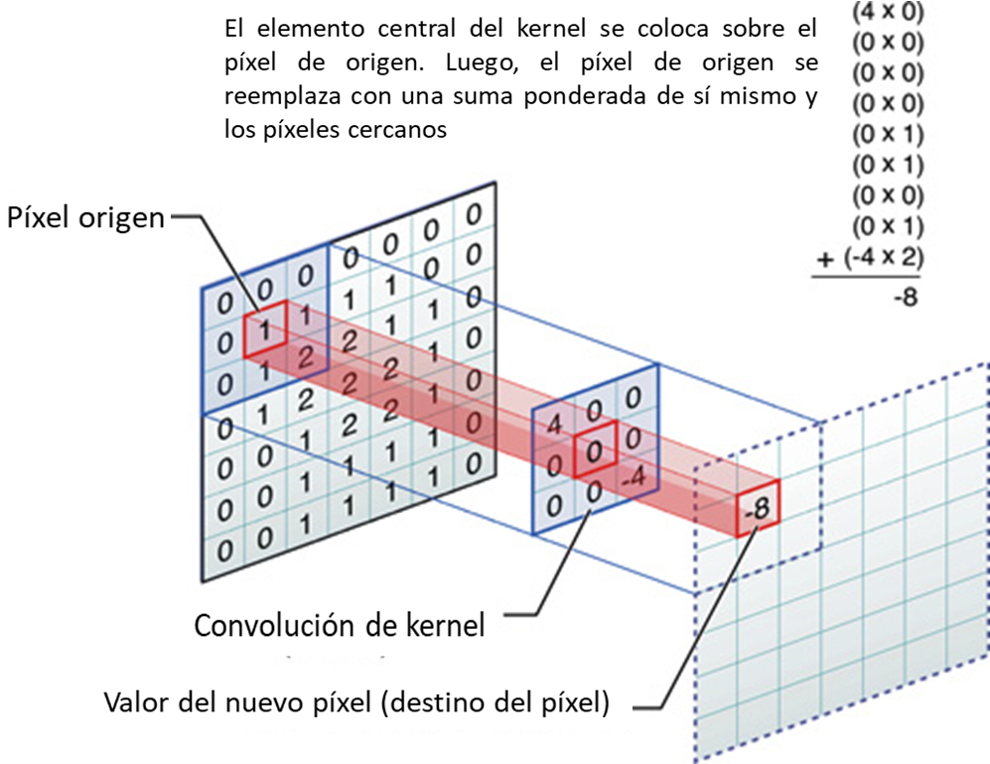
\includegraphics[scale=0.5]{Figures/Convolucion.png}
    \caption{Ejemplo de convolución del kernel, tomado de la información de la referencia \cite{developer}}
    \label{convolucion1}
\end{figure}

En la investigación desarrollada por Kim \cite{kim}, realizan el tratamiento de imágenes a blanco y negro (escala de grises) mediante la convolución del kernel \textit{Sobel}, el cual permite detectar los bordes verticales y horizontales en una imagen, obteniendo así el relieve de la imagen. En el programa R, mediante la función \texttt{magik()}, se pueden realizar el procesamiento a las imágenes y con la función \texttt{image\_convolve()} se pueden realizar la convoluciones de kernel. En la figura \ref{convolucionpractica} se muestra el resultado de aplicar la convolución con el kernel \textit{Sobel} a una imagen. En la documentación de Thyssen \cite{ImageMagick} se encuentran más ejemplos de \texttt{convolve} con varios kernels disponibles. Además de aplicaciones como el relieve de la imagen, se pueden utilizar filtros para eliminar señales e imágenes (ruido). Diferentes filtros pueden lograr este propósito y el óptimo a menudo, depende de los requisitos particulares de la aplicación que se requiera.

\begin{figure}[h]
    \begin{center}
    \captionsetup{justification=centering}
    \begin{subfigure}[b]{0.4\textwidth}
        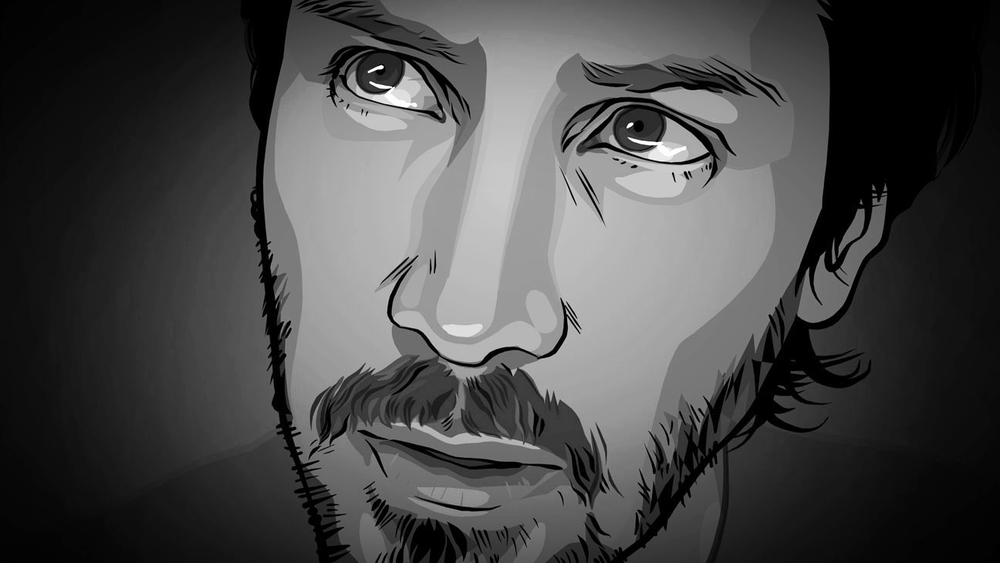
\includegraphics[scale=0.22]{Figures/darkly.jpg}
        \caption{Imagen antes de la convolución. \\ Fuente: \textit{A Scanner Darkly (2006)}.}
    \end{subfigure}
    \begin{subfigure}[b]{0.4\textwidth}
        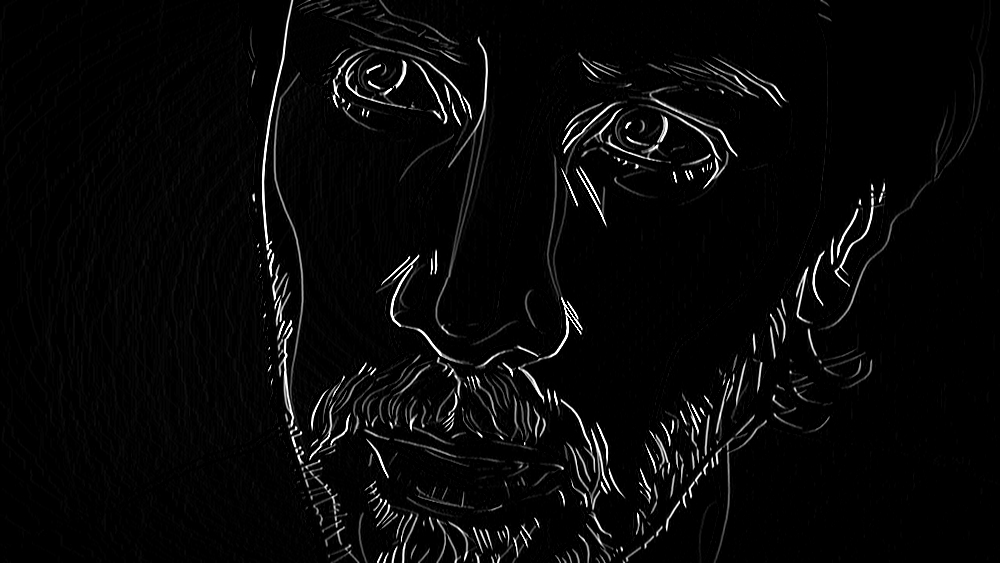
\includegraphics[scale=0.22]{Figures/imagenSolbe.jpeg}
        \caption{Imagen después de la convolución con el kernel \textit{Sobel}}
    \end{subfigure}
    \caption{Ejemplo de imagen aplicando convolución de kernel}
    \label{convolucionpractica}
    \end{center}
\end{figure}

De igual manera, en el trabajo de Kim \cite{kim}, presentan las expresiones matemáticas para la convolución con imágenes, determinando que, para el caso de las señales digitales, si $A{n}$ y $B{n}$ son funciones con respecto a un valor $n$ entero, entonces la convolución en un sistema unidimensional, se representa mediante la ecuación \ref{discretaseñal}:
\begin{equation} 
A{[n_{a}]} * B{[n_{b}]} = C{[n_{c}]} = \sum_{\tau=0}^{n_{a}-1} A[\tau] \times B{[n_{c}-\tau}],
\label{discretaseñal}
\end{equation}
\noindent donde $0 \leq n_{c} < n_{a} + n_{b} - 1$ y $\tau$ es la variable sobre la cual se realiza el desplazamiento.

Sin embargo, debido a que las imágenes son bidimensionales, es neceario la extensión a $2$-D de la ecuación \ref{discretaseñal} para realizar la convolución con imágenes, la cuál es mostrada en la ecuación \ref{discretabi}:
\begin{equation} 
A{[i_{a}, \, j_{a}]} * B{[i_{b}, \, j_{b}]} = C{[i_{c}, \, j_{c}]} = \sum_{\tau_{1}=0}^{i_{a}-1} \sum_{\tau_{2}=0}^{j_{a}-1} A[\tau_{1}, \, \tau_{2}] \times B{[i-\tau_{1}, \, j-\tau_{2}}]. 
\label{discretabi}
\end{equation}

En conclusión, gran parte de la tecnología que existe hoy en día no sería posible sin un medio para extraer información y manipular señales digitales, donde uno de los métodos para procesar imágenes digitales, llamado filtrado, se puede utilizar para reducir la información de la señal no deseada (ruido) o extraer información como los bordes de la imagen, lo cual se logra mediante un enfoque matemático utilizando la convolución y la matriz del kernel.  

El código empleado para el tratamiento de las imágenes en el software R versión 4.0.2 \cite{r} se encuentra en el repositorio GitHub \cite{github}.

\section{Aplicación de la prueba de chi cuadrada ($\chi^{2}$)}

Chi cuadrada ($\chi^2$) es la distribución de la suma de variables aleatorias cuadradas. Se utiliza la distribución $\chi^2$ para examinar si un conjunto de datos \textbf{difiere} de forma estadísticamente significativa de lo esperado, se conoce también como una prueba de calidad de ajuste y se requiere conocer la distribución que se espera ver y las frecuencias observadas de cada valor posible \cite{notasElisa}. Se utiliza la ecuación \ref{chi} para determinar el valor de $\chi^{2}$, donde $k-1$ son grados de libertad:
\begin{align} 
  \sum_{k} \frac{(\text{esperada-observada})^2}{\text{esperada}} & \sim \chi^2(|k|-1). \label{chi} \\  \nonumber
\end{align}
%$k$ es el número de categorías y 
En el tema de tesis que actualmente se desarrolla, se utiliza un GRASP (abreviatura de \textit{greedy randomized adaptive search procedures}) reactivo para hallar la solución al  problema. Este algoritmo depende de un valor alfa ($\alpha$) para construir la solución. Para la afinación del parámetro $\alpha$ se decidió utilizar una estrategia reactiva en la cual el valor de $\alpha$ se adapta dinámicamente según los resultados obtenidos en las iteraciones previas, por lo tanto, se utiliza un conjunto discreto de valores predeterminados de alfas $A = \{\alpha_{1},\, \alpha_{2}, \, \dots, \alpha_{k}\}$.

En la experimentación llevada a cabo para la tesis, se tiene en total de $k=10$ valores de alfa diferentes y se ejecutaron $n=1,000$ iteraciones del algoritmo para cada instancia, actualizando la probabilidad de selección para cada alfa cada $100$ iteraciones. Para la aplicación de la prueba $\chi^2$ se plantea como hipótesis nula ($H_{0}$) que las alfas en cada instancia son seleccionadas con la misma probabilidad y, como hipótesis alternativa ($H_{1}$) que las alfas en cada instancia no son seleccionadas con la misma probabilidad.

En el cuadro \ref{tablacontingencia}, se muestra la tabla de contingencia para la aplicación de la prueba $\alpha$. La frecuencia de cada alfa se tomó de los resultados arrojados por el algoritmo y el valor esperado de cada alfa se determinó mediante la ecuación \ref{probabilidad}:
\begin{align} 
  \text{Frecuencia esperada} & = P(\alpha) \times \text{n} \label{probabilidad} \\ 
    \text{Frecuencia esperada} & = \frac{1}{10} \times 1000 \\  \nonumber
    \text{Frecuencia esperada} & = 100. \\  \nonumber
\end{align}

\begin{table}
\centering
\caption{Tabla de contingencia para la prueba $\chi^2$}
\begin{tabular}{|c|r|r|r|r|r|}
\hline
\multirow{2}{*}{\textbf{Alfa}}       & \multicolumn{2}{c|}{\textbf{Frecuencia}}                                                                                                                       & \multicolumn{3}{c|}{\textbf{Diferencia cuadrada}}                                            \\ \cline{2-6} 
                                     & \multicolumn{1}{c|}{\begin{tabular}[c]{@{}c@{}}Observada\\ ($E$)\end{tabular}} & \multicolumn{1}{c|}{\begin{tabular}[c]{@{}c@{}}Esperada\\ ($E$)\end{tabular}} & \multicolumn{1}{c|}{E-O} & \multicolumn{1}{c|}{$(E-O)^2$} & \multicolumn{1}{c|}{Normalizada} \\ \hline
0.06                                 & 105                                                                            & 100                                                                           & -5                       & 25                             & 0.25                             \\ \hline
0.07                                 & 99                                                                             & 100                                                                           & 1                        & 1                              & 0.01                             \\ \hline
0.08                                 & 113                                                                            & 100                                                                           & -13                      & 169                            & 1.69                             \\ \hline
0.09                                 & 124                                                                            & 100                                                                           & -24                      & 576                            & 5.76                             \\ \hline
0.10                                 & 110                                                                            & 100                                                                           & -10                      & 100                            & 1                                \\ \hline
0.15                                 & 90                                                                             & 100                                                                           & 10                       & 100                            & 1                                \\ \hline
0.20                                 & 106                                                                            & 100                                                                           & -6                       & 36                             & 0.36                             \\ \hline
0.25                                 & 84                                                                             & 100                                                                           & 16                       & 256                            & 2.56                             \\ \hline
0.30                                 & 82                                                                             & 100                                                                           & 18                       & 324                            & 3.24                             \\ \hline
0.35                                 & 87                                                                             & 100                                                                           & 13                       & 169                            & 1.69                             \\ \hline
\multicolumn{1}{|l|}{\textbf{Total}} & \textbf{1,000}                                                                 & \textbf{1,000}                                                                & \textbf{0}               & \textbf{1,756}                 & \textbf{17.56}                   \\ \hline
\end{tabular}
\label{tablacontingencia}
\end{table}

Para ejecutar la prueba de $\chi^{2}$ se utilizó la función \texttt{chisq.test()} del programa R, obteniendo como resultado un  $\chi^{2} \thickapprox 17.56$ con $9$ grados de libertad y un valor $p$ = $0.040$, por lo cual se procede a \textit{rechazar} la hipótesis nula con un nivel de confianza del $95\%$, lo que implica que al parecer se está seleccionando con mayor frecuencia algún valor de alfa dentro del conjunto dado. Este resultado tiene mucha lógica, ya que el algoritmo va seleccionando con mayor frecuencia aquellos valores de alfa que presentan mejor desempeño. El código empleado en el software R versión 4.0.2 para la prueba de chi cuadrada ($\chi^{2}$) se encuentra en el repositorio GitHub \cite{github}.

\VerbatimInput{chi.txt}

\section{Demostraciones numérica y analítica}

Sea $X$, $Y$ variables aleatorias y $a$, $b$, $c$, $d$ son constantes conocidas, demostrar que:

\begin{enumerate}[(a)]
    \item Cov($aX + b, \, cY + d$) = $ac$Cov[($X, \, Y$].
    \item Var[$X + Y$] = Var[$X$] + Var[$Y$] + 2Cov[$X,Y$].
\end{enumerate}

\noindent Con base en el desarrollo del teorema $6.2$ y $6.4$ del libro de Grinstead \cite{librop}, se tiene que:
\begin{align} \label{valorEsperado}
    \nonumber
    \text{Cov}(aX + b, \, cY + d)  & = E[(aX + b)(cY + d)] - E[(aX + b)]E[(cY + d)] \\ \nonumber
    & = E(acXY + aXd + bcY + bd) − [aE(X) + b][cE(Y) + d] \\ \nonumber
    & =  acE(XY) + adE(X) + bcE(Y) + bd -[acE(X)E(Y) + adE(X) + bcE(Y) + bd] \\ \nonumber
    & =  acE(XY ) + adE(X) + bcE(Y) + bd - acE(X)E(Y) - adE(X) - bcE(Y) - bd \\ \nonumber
    & =  acE(XY) − acE(X)E(Y) \\
    & = ac\text{Cov}(X, Y).  
\end{align}

\noindent De acuerdo al desarrollo del teorema $6.6$ y $6.8$ del libro de Grinstead \cite{librop}, se tiene que:
\begin{align} \label{varianza}
    \nonumber
    \text{Var}[X + Y]  & =  E[(X + Y )^2] − [E(X) + E(Y)]^2 \\ \nonumber
    & =  E(X^2 + 2XY + Y^2) - [E(X)^2 + 2E(X)E(Y) + E(Y)^2]  \\ \nonumber
    & =  E(X^2) + 2E(XY) + E(Y^2) - E(X)^2 - 2E(X)E(Y) - E(Y)^2 \\ \nonumber
    & = E(X^2) - E(X)^2 + E(Y^2) - E(Y)^2 + 2[E(XY) - E(X)E(Y) \\ 
    & =  \text{Var}[X] + \text{Var}[Y] + 2\text{Cov}[X,Y]. 
\end{align}

Para la demostración numérica, se generaron $100$ valores aleatorios para $X$ y $Y$ (donde no necesariamente son independientes) y se estableció $a=5$, $b=100$, $c=20.5$ y $d=0.85$. Se realizaron $100$ replicas aplicando las ecuaciones \ref{valorEsperado} y \ref{varianza}, donde $X$ y $Y$ tenían diferente tipo de distribución (uniforme, normal, exponencial y Poisson). Los resultados de la simulación para la covarianza y varianza de estos valores se muestran en las figuras \ref{resultadosValorE} y \ref{resultadosVar}, respectivamente, en las que se puede observar que se cumple la igualdad de las ecuaciones \ref{valorEsperado} y \ref{varianza}, respectivamente, sin importar el tipo de distribución y o la independencia de variables aleatorias $X$ y $Y$ (ver figuras \ref{resultadosValorEdep} y \ref{resultadosVardep}). 

\begin{figure}[h]
    \begin{center}
    \captionsetup{justification=centering}
    \begin{subfigure}[b]{0.5\textwidth}
        \includegraphics[scale=0.35]{Figures/norm-pois.png}
        \caption{Con $X \sim N(\mu, \, \sigma)$ y $Y \sim Pois(\lambda)$}
    \end{subfigure}
    \begin{subfigure}[b]{0.5\textwidth}
        \includegraphics[scale=0.35]{Figures/unif-exp.png}
        \caption{Con $X \sim U(0,1)$ y $Y\sim Exp(\lambda)$}
    \end{subfigure}
        \begin{subfigure}[b]{0.5\textwidth}
        \includegraphics[scale=0.35]{Figures/exp-pois.png}
        \caption{Con $X \sim Exp(\lambda)$ y $Y \sim Pois(\lambda)$ + $X$}
        \label{resultadosValorEdep}
    \end{subfigure}
    \caption{Resultados simulación para la covarianza}
    \label{resultadosValorE}
    \end{center}
\end{figure}

\begin{figure}[h]
    \begin{center}
    \captionsetup{justification=centering}
    \begin{subfigure}[b]{0.5\textwidth}
        \includegraphics[scale=0.35]{Figures/var-norm-pois.png}
        \caption{Con $X \sim N(\mu, \, \sigma)$ y $Y \sim Pois(\lambda)$}
    \end{subfigure}
    \begin{subfigure}[b]{0.5\textwidth}
        \includegraphics[scale=0.35]{Figures/var-unif-exp.png}
        \caption{Con $X \sim U(0,1)$ y $Y\sim Exp(\lambda)$}
    \end{subfigure}
    \begin{subfigure}[b]{0.5\textwidth}
        \includegraphics[scale=0.35]{Figures/var-exp-pois.png}
        \caption{Con $X \sim Exp(\lambda)$ y $Y \sim Pois(\lambda)$ + $X$ }
         \label{resultadosVardep}
    \end{subfigure}
    \caption{Resultados simulación para la varianza}
    \label{resultadosVar}
    \end{center}
\end{figure}

Todas las simulaciones fueron realizadas en el software R versión 4.0.2 y el código empleado se encuentra en el repositorio GitHub \cite{github}.

\bibliography{refProbabilidad}
\bibliographystyle{plain}

\end{document}
